\chapter{Methods}\label{ch3:methods}

The objective of this work is to freely rerender concurrent one-on-one video chat frames from the points of view of both participants bidirectionally and in real-time. This would help simulate the experience of conversing face-to-face with a person in the real world. We adopted Tucker and Snavely's~\cite{single_view_mpi} single-view MPI network, for it is the state-of-the-art open-source single-view view synthesis network, to the best of our knowledge. When we initially ran the publicly available inference part of the network on a video chat frame, we found that the generated disparity map (Equation~\ref{eq:disparity-map}) was visually inaccurate. Comparatively (Figure~\ref{fig:great-off-kilter-disparity}), the inferred disparity map would be much more visually accurate whenever a real estate video frame was processed. The latter outcome is to be expected because Tucker and Snavely's model was originally trained on RealEstate10K~\cite{zhou2018stereo} video dataset. Specifically, even though the picture quality of synthesized views would be brilliant for both categories of video frames by virtue of the model having been efficiently tweaked and extensively trained by the authors (given contemporary hardware limitations), yet synthesized video-chat-related frames alone would seem unnaturally concave/convex at arbitrary positions within each rerendered frame, not to mention the loss of perspectivity and the induction of random distortions occurring within the frame as well.

\begin{figure}[!h]
    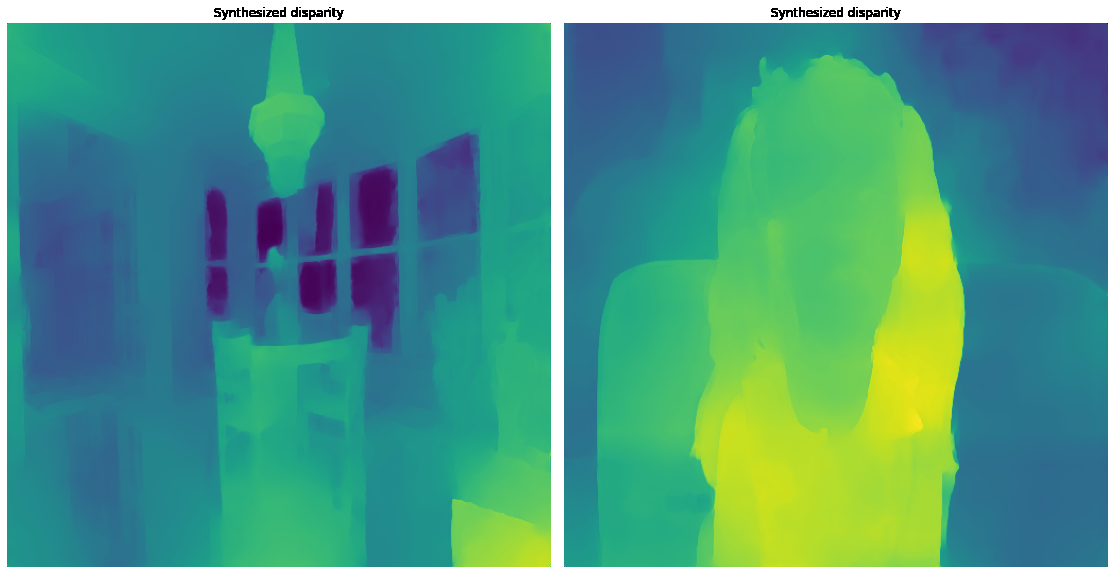
\includegraphics[width=1\columnwidth]{figures/great-off-kilter-disparity.png}
    \caption{Disparity Heat Maps Synthesized by Tucker and Snavely's model~\cite{single_view_mpi} for Real Estate and Video Chat Frames}
    \label{fig:great-off-kilter-disparity}
    {\small The disparity map on the left encodes a real estate scene and the one on the right, a video chat scene. The real estate map successfully shows appropriate heat/depth gradations from the hottest/closest armrest region on the bottom right to the coldest window regions at the back. The video chat map, on the other hand, counterintuitively shows that the face of the girl in the scene is situated behind the body, and the couch is somehow disjointed.}  
\end{figure}

\section{Approach}\label{sec:approach} 

As a primary step (Figure~\ref{fig:mpi-training-pipeline}), we attempted to increase Tucker and Snavely's depth prediction accuracy for video-chat-relevant frames containing close-up shots of people, so we may see a drastic reduction in the number of artifacts induced in synthesized frames. This involved curating and utilizing both RealEstate10K and MannequinChallenge~\cite{li2019learning} datasets. The latter contains video frames that resemble video chat scenes, as it is composed solely of scenes of people pretending to be mannequins while a camera moves around them, flowing seamlessly from scene to scene. Essentially, we performed transfer learning~\cite{radhakrishnan_what_2019} with the pretrained weights of Tucker and Snavely's model by \textit{fine-tuning}/\textit{refitting} them to a dataset other than the one they were originally trained on. Secondly (Figure~\ref{fig:3d-video-chat-rendering-pipeline}), we introduced the head pose detection submodule of OpenFace 2.2~\cite{baltrusaitis_openface_2018} into the inference pipeline of Tucker and Snavely, so that ``\textit{viewee}" video frames may be rerendered at the head pose obtained from ``\textit{viewer}" frames. We considered a few state-of-the-art open-source head pose estimation models, including WHENet~\cite{zhou_whenet_2020} for its speed and consistency, and ultimately chose OpenFace 2.2 because it works well with the Deep Learning (DL) framework used by Tucker and Snavely (TensorFlow 2.2) and can be installed in the same dockerized environment as COLMAP~\cite{schoenberger2016sfm,schoenberger2016mvs} and the rest of the dependencies needed by our comprehensive pipeline. 

\begin{figure}[!h]
    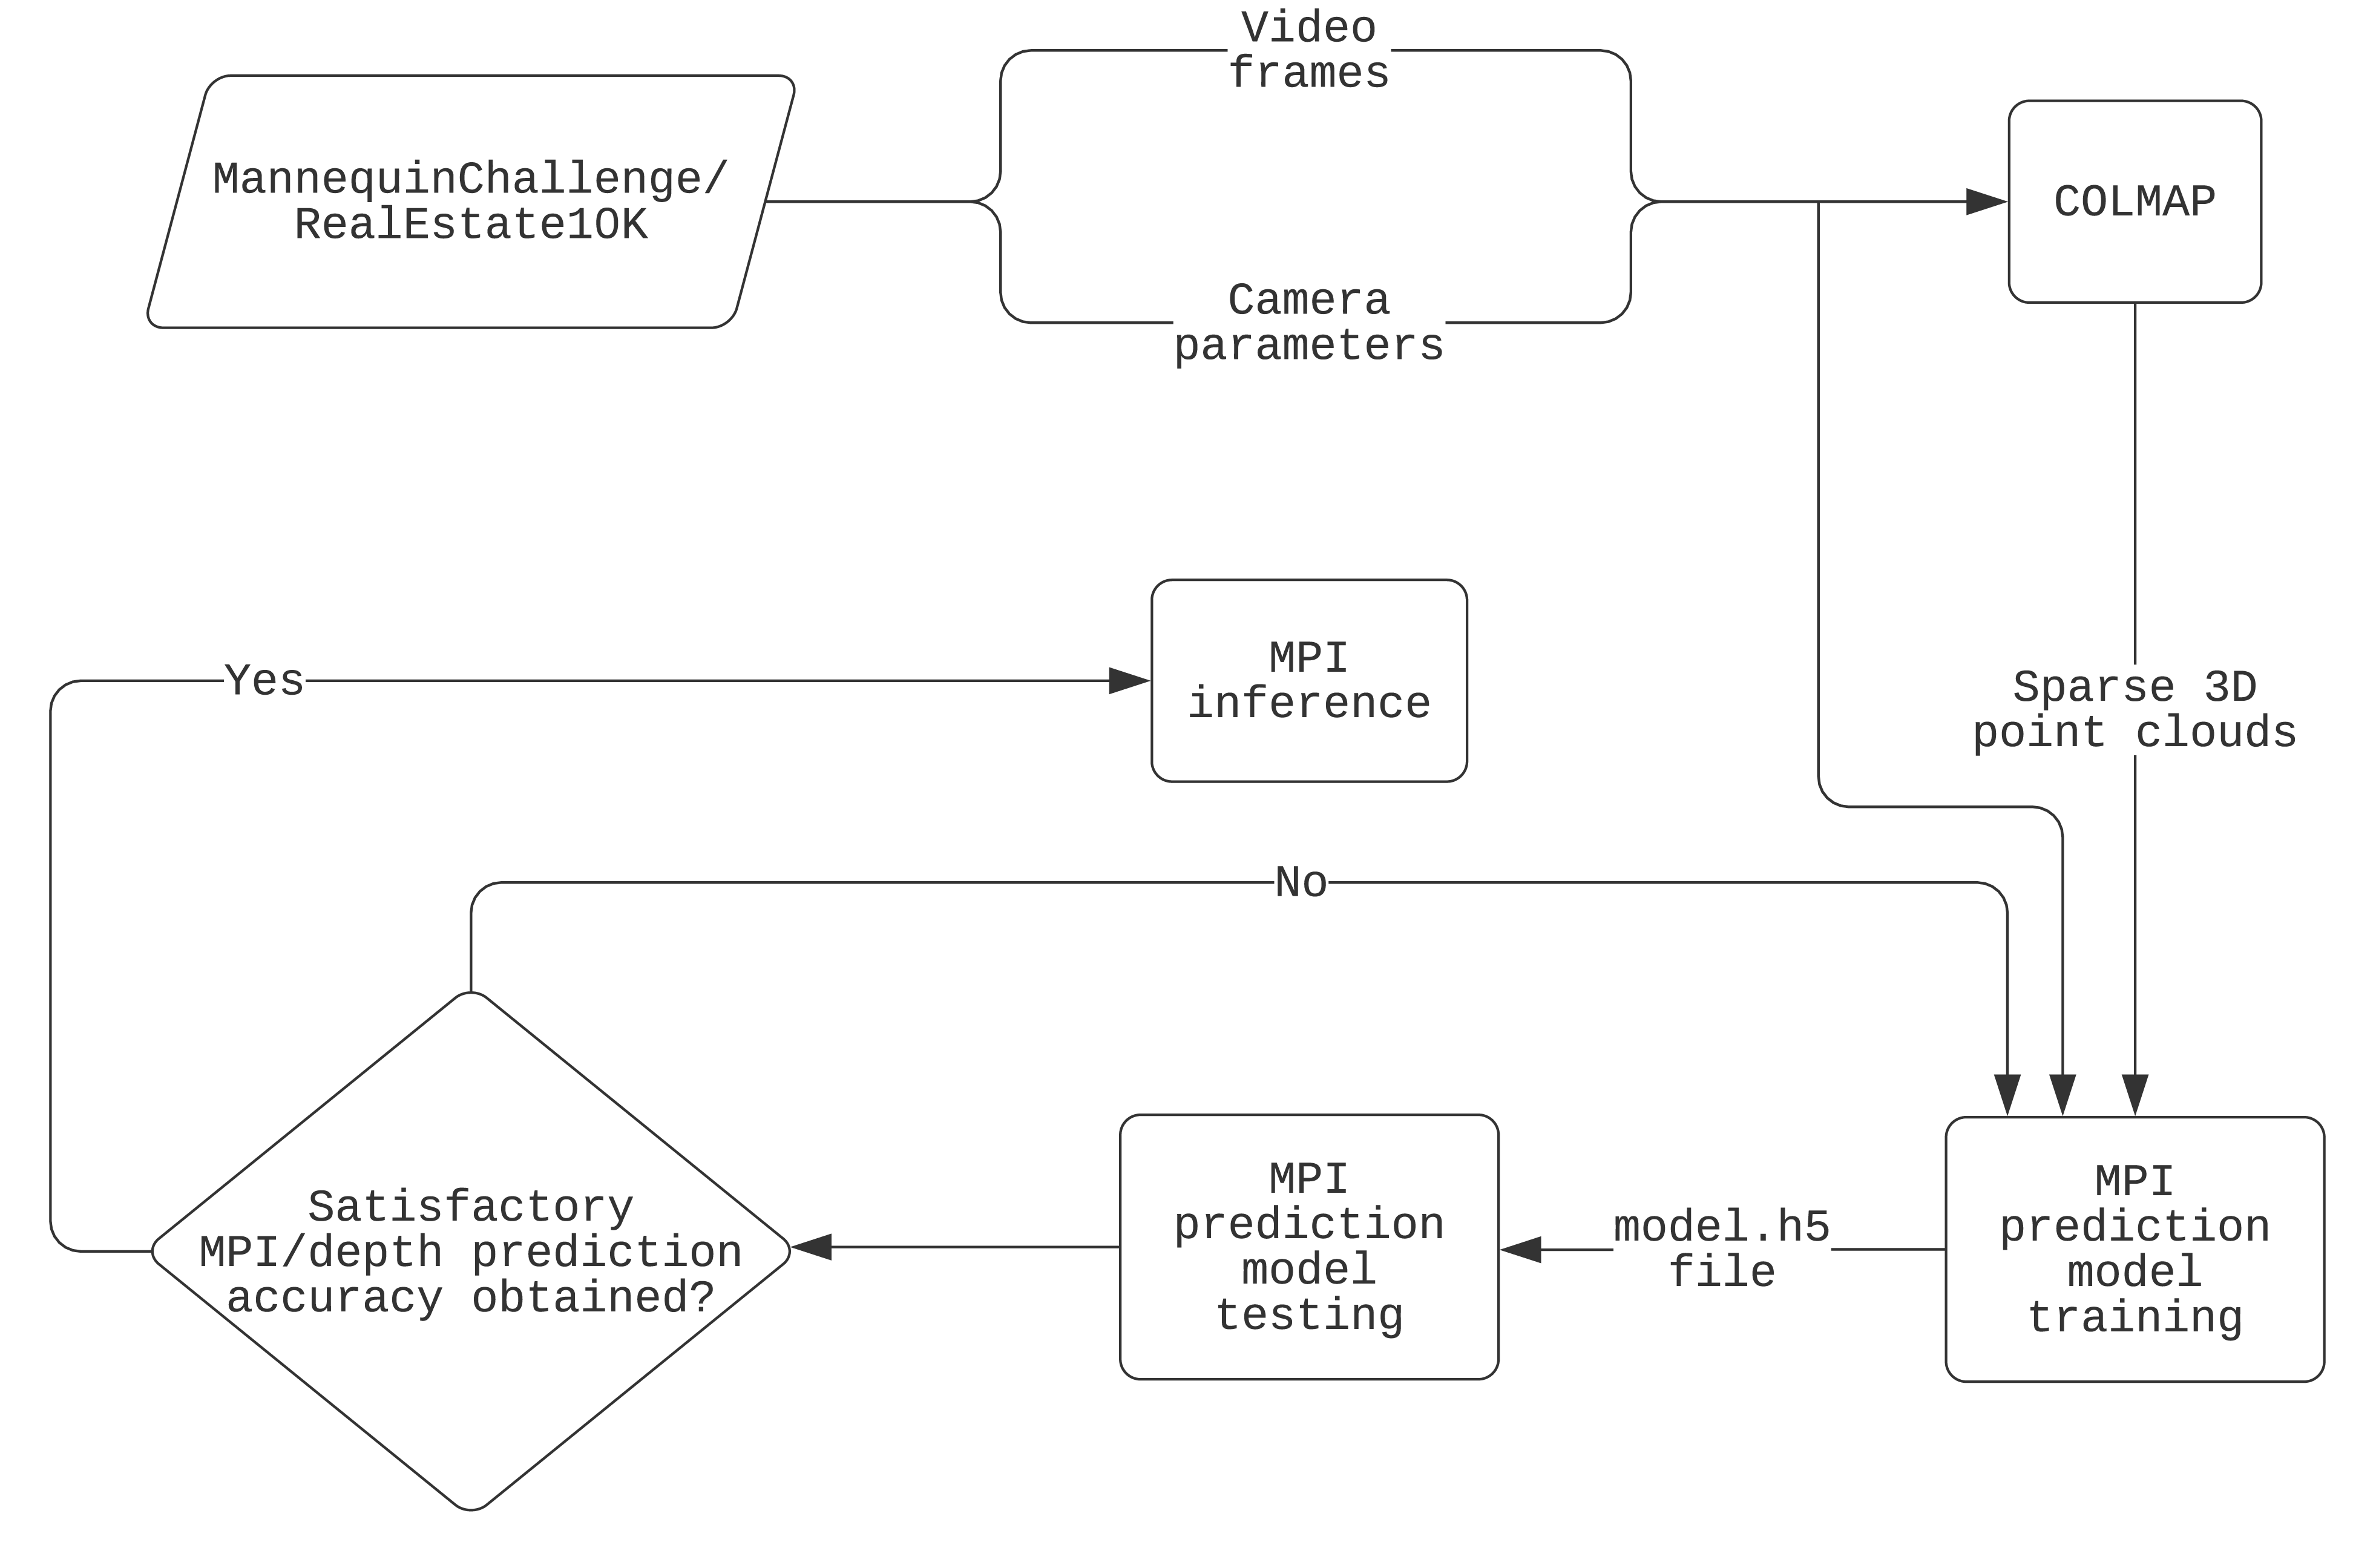
\includegraphics[width=1\columnwidth]{figures/mpi-training-pipeline.png}
    \caption{MPI Training Pipeline}
    \label{fig:mpi-training-pipeline}
\end{figure}

As inference is one of the only parts of the network made publicly available by Tucker and Snavely~\cite{single_view_mpi} due to the proprietary nature of some other aspects of their implementation, we went about recreating Tucker and Snavely's DispNet-like model~\cite{mayer_large_2016} first before retraining it on requisite datasets and repurposing it for video chat view synthesis. We recreated parts of the model from the code released (Section~\ref{sec:code-sources}) by the authors involving their network definition (convolutional layers, kernel sizes, etc.), and the code used by them for rendering views from new camera positions with homographies and related operations (Equation~\ref{eq:rerendered-target}). We then put together other aspects of the network that called for a more involved recreation process like the data loader part and the loss functions (Equation~\ref{eq:aggregate-loss}). Requisite components of input data, including point clouds, had to be extracted and loaded in. One of the key features of Tucker and Snavely is to use sparse point cloud data to make the view synthesis loss scale-invariant (Subsection~\ref{subsec:base-papers}). To obtain such inputs, we processed both datasets with COLMAP and wrote a custom data loader. We took inspiration from Zhou et al.'s~\cite{zhou2018stereo} stereo MPI paper for building the data loader, for the code they tailored to load in data (Section~\ref{sec:code-sources}) was refactored and reused by Tucker and Snavely as well. Their implementations of subsequence selection and random cropping proved useful.

\begin{figure}[!h]
    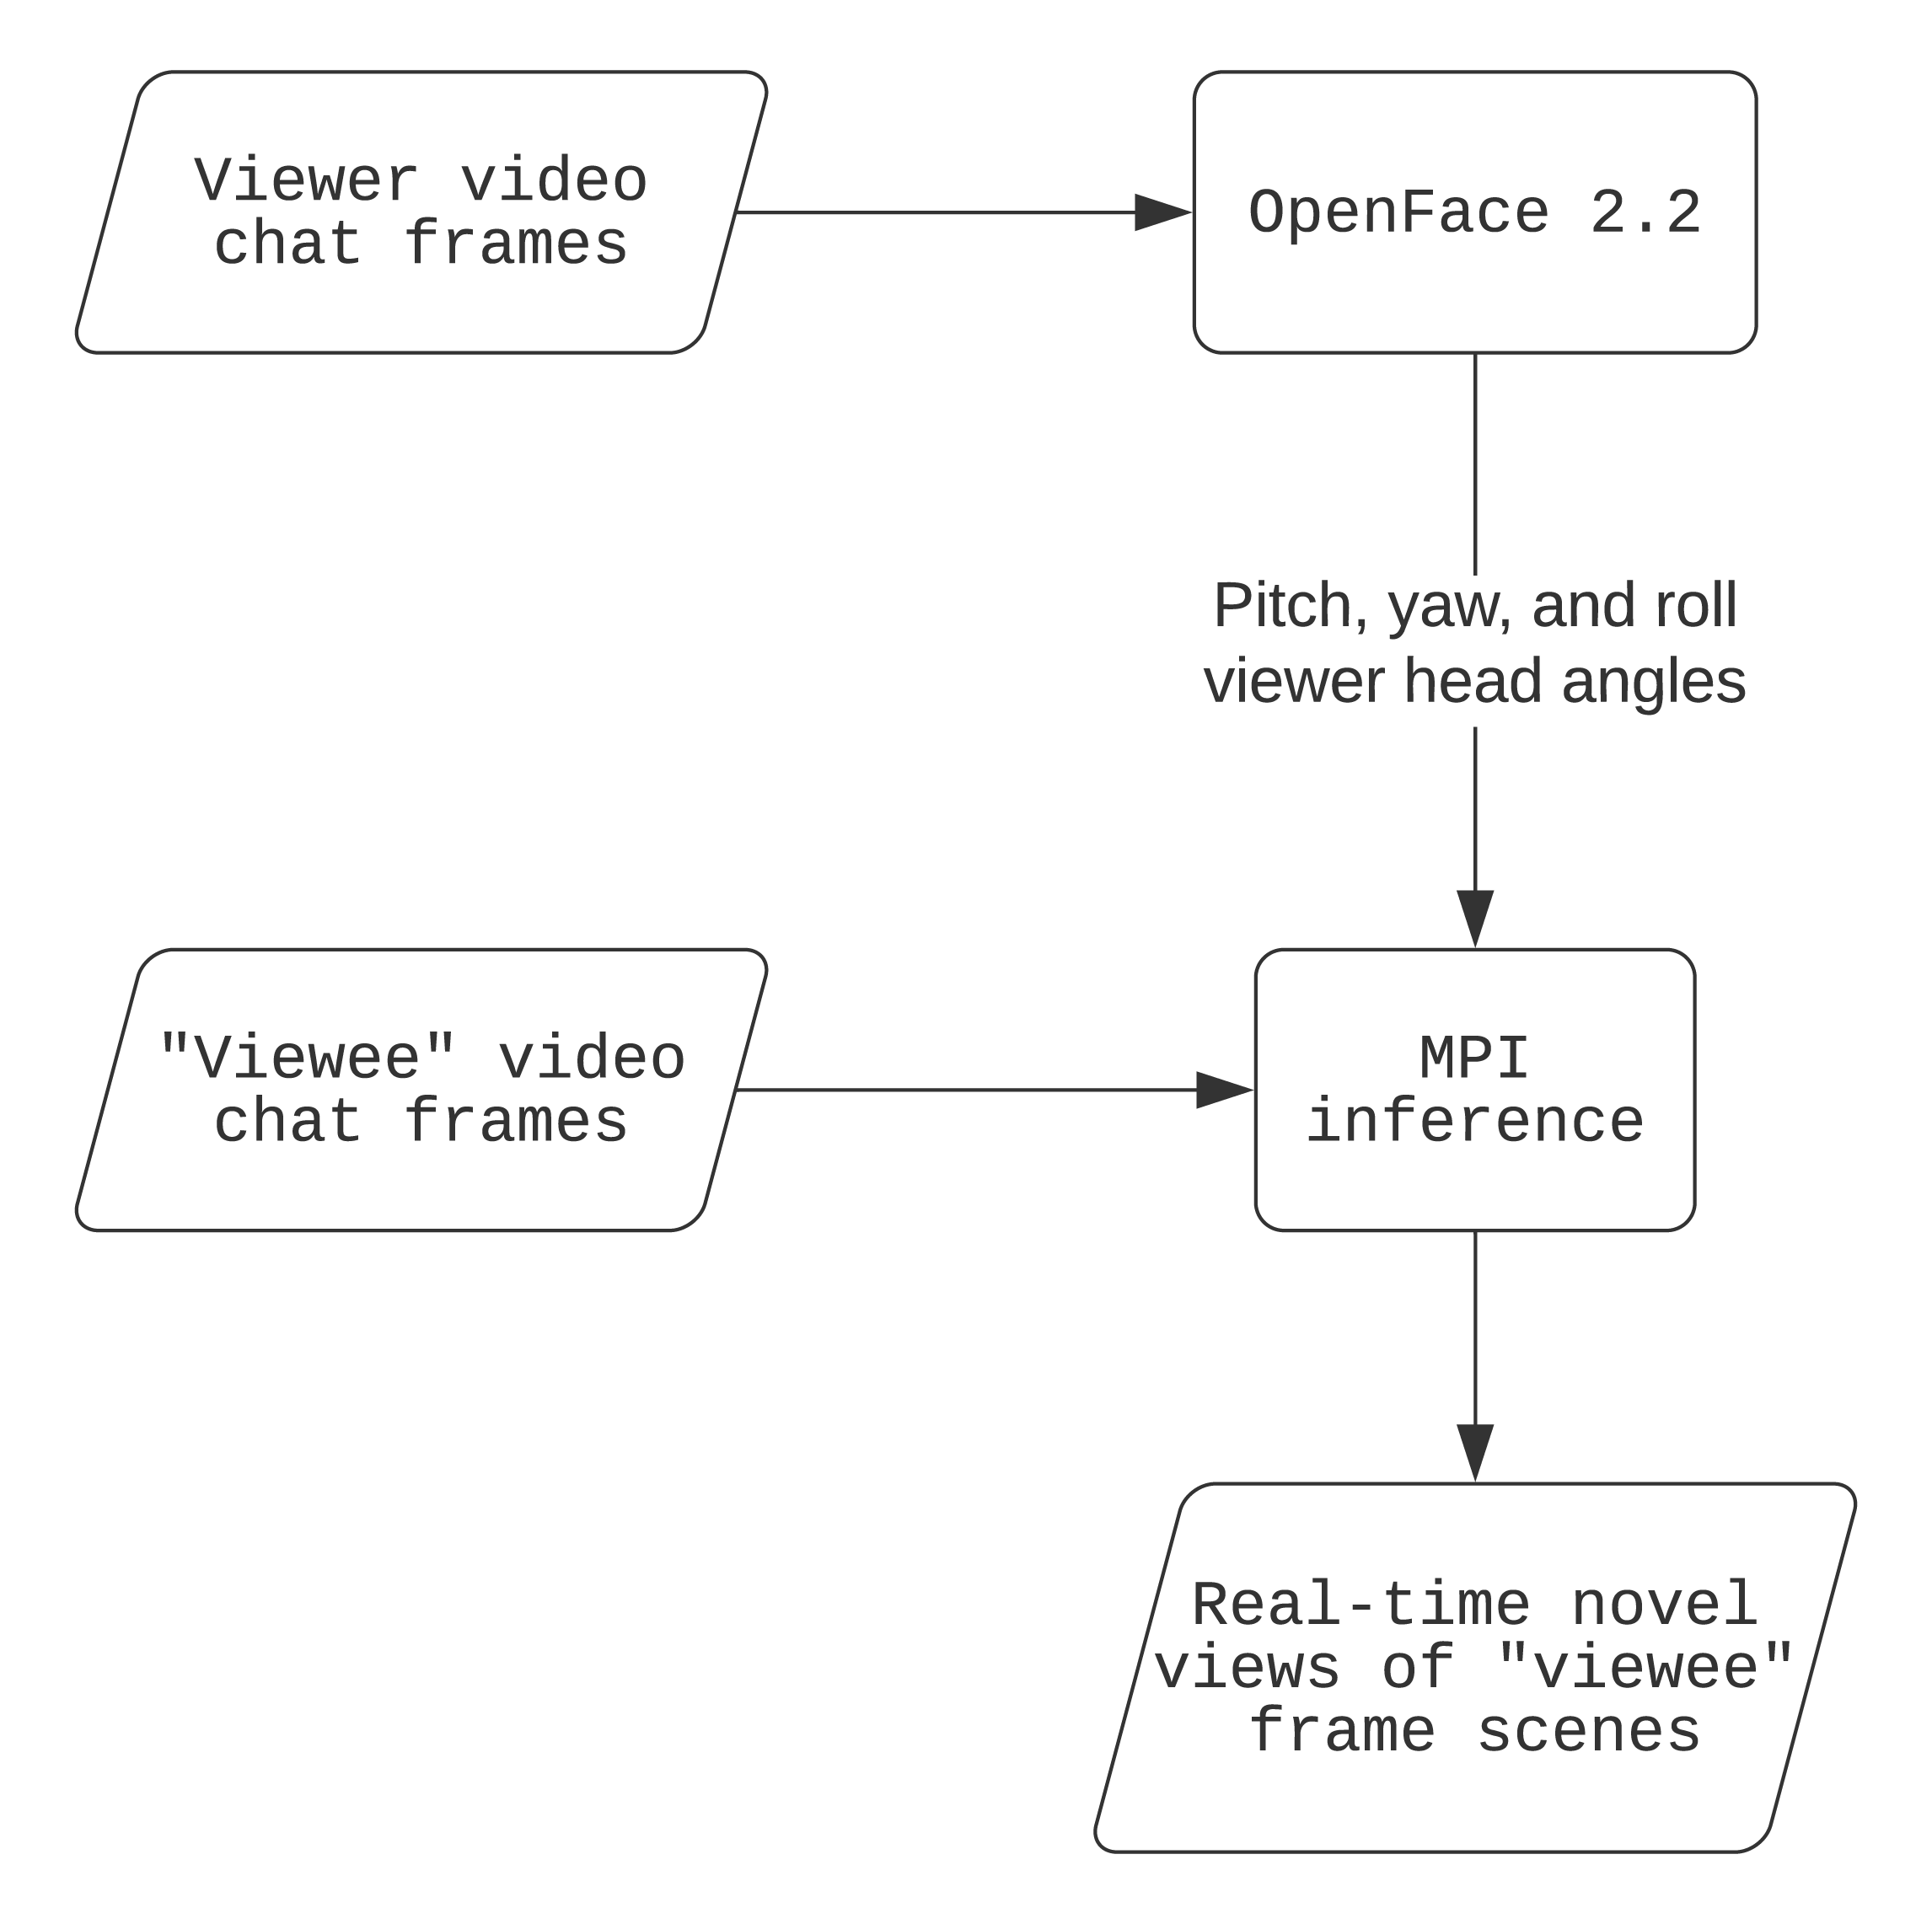
\includegraphics[width=0.60\columnwidth]{figures/3d-video-chat-rendering-pipeline.png}
    \caption{3D Video Chat Rendering Pipeline}
    \label{fig:3d-video-chat-rendering-pipeline}
\end{figure}

We retrained the recreated network twice, separately. One variant was fine-tuned exclusively on the video-chat-relevant MannequinChallenge video dataset~\cite{li2019learning} which is $\sim$96\% smaller than RealEstate10K in training data, as of this writing. The other variant was retrained on a combination of both datasets by having the model pick equal batches of frames randomly and alternatingly between both datasets. We considered addressing this inherent data imbalance problem by making the model pick an appropriate proportion of RealEstate10K frames for every MannequinChallenge frame randomly selected, but ultimately voted against it in favor of resolving more pressing issues such as the training errors mentioned in section~\ref{sec:implementation}. We are grateful to the authors of Tucker and Snavely for forewarning us that there is a risk of overfitting to the much smaller MannequinChallenge dataset, even though it was generally mentioned in both Zhou et al. and Tucker and Snavely that the stereo and single-view models were generalizable to domains besides real estate footage. Hence, we felt the need for deploying the second variant to help access this risk. We could also have taken another transfer learning route of freezing all but the last few layers of the model to possibly reduce overfitting but we chose to unfreeze all layers in favor of making the variants wholly robust. We stack up these variants to each other and also to the pretrained single-view model and compare their performances in chapter~\ref{ch4:experiments-results}. Next, after introducing the head pose estimation API of OpenFace 2.2 into the inference pipeline of the variants, we converted estimated head orientations into a form amenable to rendering with MPIs. This involved manipulating yaw, pitch, and roll head angles. We also visually verified for if the rerendered frames were getting seemingly aligned with the extracted head poses or not.

\section{Data}\label{sec:data} 

Both Mannequin Challenge~\cite{li2019learning} and RealEstate10K~\cite{zhou2018stereo} datasets were created by roughly the same group of researchers hailing from Google. They involved the same ORB-SLAM2, COLMAP, and scale-normalization procedures of Zhou et al.~\cite{zhou2018stereo} (Subsection~\ref{subsec:base-papers}). Hence, both datasets consist of the same kind of metadata in text files pertaining to the downloadable videos. Each text file begins with the video’s YouTube link on the first line and continues with the details of each COLMAP-processed video frame from the second line onward. Frame details include the timestamp (in microseconds), camera intrinsics, and camera extrinsics. As mentioned in subsection~\ref{subsec:base-papers}, COLMAP is a 3D scene reconstruction pipeline. It attempts to recover the 3D scene structure from even those unstructured 2D images of the scene that do not come tagged with any prior knowledge of camera intrinsics, extrinsics, and nature of objects captured. The extracted scene structure is either in the form of sparse 3D points along with the camera parameters for each input 2D image or in the form of dense 3D points with associated color information. COLMAP's pipeline can be given by: feature detection $\rightarrow$ pairwise feature matching  $\rightarrow$ correspondence estimation $\rightarrow$ incremental structure from motion (Figure~\ref{fig:colmap-photogrammetry-pipeline}). Fortunately, absolute camera poses are not required by the model; only the relative ones made available with the help of COLMAP in these text files are. Our scripts to download and curate all these videos were facilitated by our compilation of a comprehensive Docker container ensuring robustness in code reusability and transferability. Resolving version compatibility issues among our project dependencies such as COLMAP and OpenFace 2.2, both in the Docker container and in Google Colaboratory proved paramount to the successful running of our experiments. All our scripts, notebooks, sample renderings, demos, and most other aspects of our code for this project can be found in our GitHub repository (Section~\ref{sec:code-sources}).

\begin{figure}[!h]
    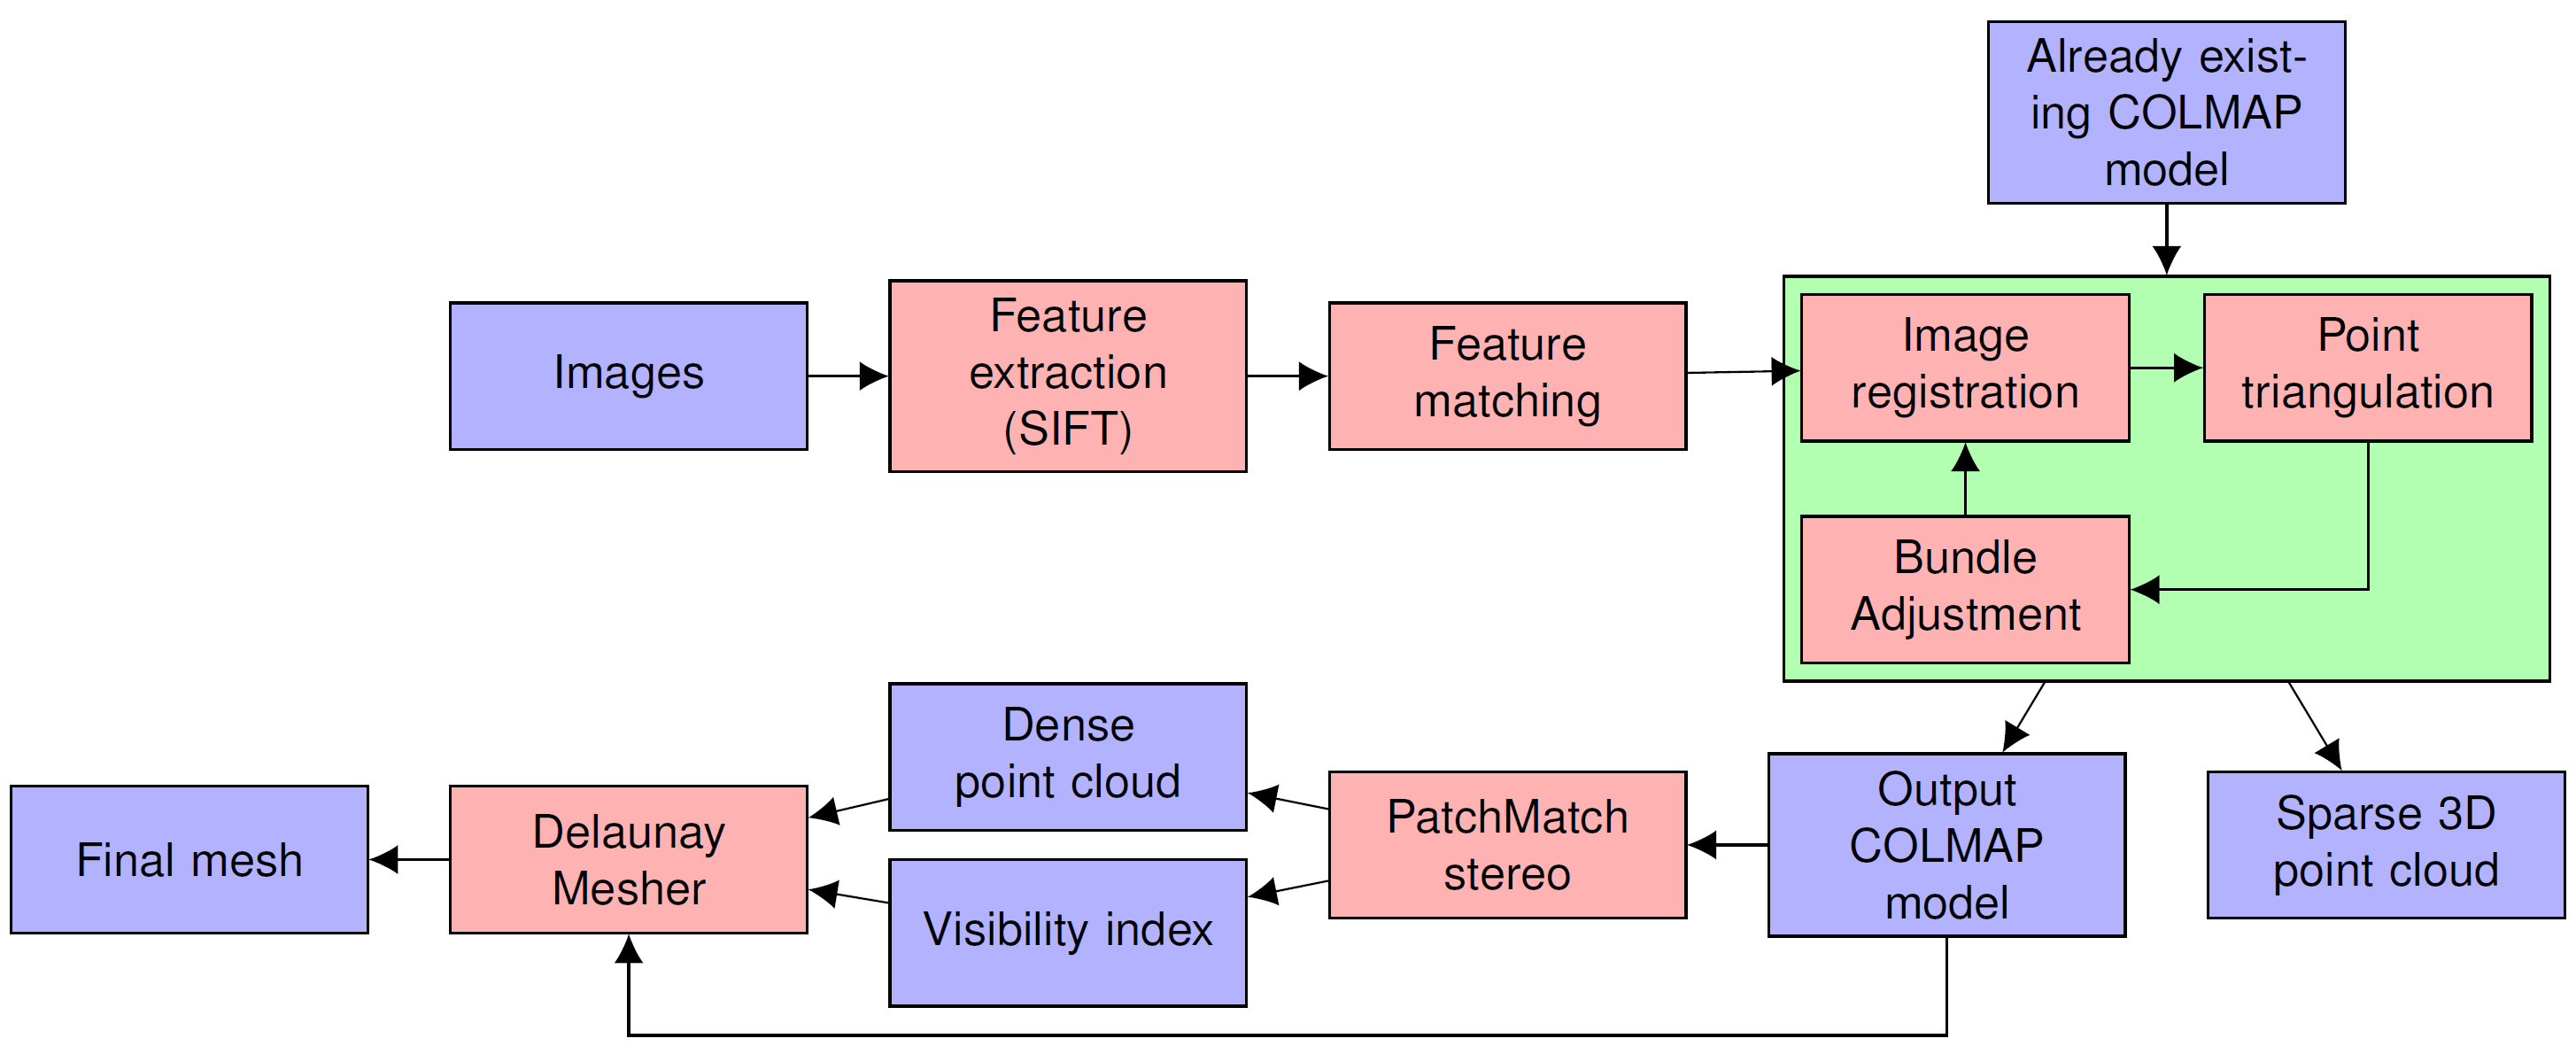
\includegraphics[width=1\columnwidth]{figures/colmap-photogrammetry-pipeline.png}
    \caption{Photogrammetry workflow used in COLMAP~\cite{pinard_does_2021}}
    \label{fig:colmap-photogrammetry-pipeline}
\end{figure}
    
Although our training and testing scripts are designed to crop all incoming video frames to 512$\times$512 pixels, we ensured that we downloaded all videos with youtube-dl at 720p resolution. This uniformity was so we could reduce the number of sources of arbitrariness in the initial process of replicating Tucker and Snavely's~\cite{single_view_mpi} work. Linking youtube-dl with the download management utility aria2~\cite{noauthor_aria2_2021} proved very useful in bolstering youtube-dl’s download speed by optimizing resource utilization. We then targeted addressing youtube-dl download errors. There would inevitably be several partial and/or skipped downloads for various reasons ranging from the videos being taken down from YouTube over time to fixable errors intrinsic to youtube-dl. Moreover, some videos were unavailable in their 720p versions and were discarded by us with the aim of maintaining consistency. In favor of maintaining the pristine versions we chose not to manually convert the varying resolutions to 720p. Although differently scaled videos should theoretically not pose any problem to training or to 3D point cloud generation with COLMAP, we opted again to go with uniformity and consequent ease of reproducibility for one and all.
    
We were finally able to procure 66,861 RealEstate10K videos with 9,095,528 frames and 2,364 MannequinChallenge videos with 117,811 frames, for processing. But not all downloaded videos could be processed. For instance, only $\sim$60000 RealEstate10K videos were actually COLMAP-processed and used for training. This is because the rest of the videos did not meet COLMAP processing requirements. And, it would have taken 200 days to process all 66,861 videos with COLMAP with CPUs alone. Fortunately, we were able to avail the benefits NVIDIA Tesla V100 GPUs (rated the best server models in 2020) at Cal Poly and could bring down the processing time to 25 days. In these ways, we obtained the required points clouds and frames for both training and testing.
















\section{Implementation}\label{sec:implementation} 

We attempted to generate accurate MPI representations for close-up targets such as heads and upper bodies, and improve the pixel accuracies of views synthesized from these MPIs. After putting together the data loader to feed the datasets and point clouds into the network, we recreated loss functions from the textual descriptions in the single-view MPI paper. As mentioned in subsection~\ref{subsec:base-papers}, we likened our training process to Tucker and Snavely~\cite{single_view_mpi} with regard to various aspects such as the use of TensorFlow 2.2, ADAM solver, a pixel loss weight of 1, a smoothness loss weight of 0.5, etc. We experimented with choices of learning rate and depth loss weight but generally picked 0.00001 and 1, respectively, contrary to the 0.0001 and 0.1 used in Tucker and Snavely. We reduced the learning rate because we were fine-tuning the pretrained model rather than training from scratch. The requirement that we had to have view synthesis quality as supervision was fulfilled by taking a frame one frame apart from each chosen training frame as target ground truth. We trained for a number of steps rather than for a number of epochs. Our data loader randomizes batch picking not only for testing but also for training. Moreover, we have not yet been able to go beyond the model experimentation stage. Exposing the model to a wide variety of frames is the way to go in this stage. For the model to be training sequentially on all frames clip by clip, and covering entire datasets multiple times in multiple epochs, it should be free of any errors that impede its progress toward convergence. We have not been able to bring our model up to that stage yet. 

We used wandb.ai~\cite{wandb} for experiment tracking and it proved to be a valuable tool for our entire process. It helped us spin different variants of the model, chiefly characterized by their being trained either on MannequinChallenge alone or on a combination of both datasets. As with some notable attempts at model training in the community, we encountered Not a Number (NaN) gradient errors that took a good chunk of our resolution efforts in this work, but ultimately could not be resolved. NaN losses signal that the issue of vanishing/exploding gradients may be present. In this work, NaN gradients could only be reduced in their frequency of occurrence from once in several hundred steps to once in several thousand steps. wandb.ai helped immensely in resuming not just the training runs themselves but also the activity of logging training metrics right from the point where the run broke off due to a NaN error. What also helped bring down the frequency of encountering NaNs, we believe, was the fact that we removed all those videos from the training/testing process that had at least one frame with a point cloud composed of less than two 3D points. Our Linux command to locate such point cloud \texttt{.txt} files (Section~\ref{sec:code-snippets}) would take about 3 hours to sift through a set of 2500 point cloud directories with one \texttt{.txt} file per video frame. Replacing \texttt{cumprod} used in several places in the single-view MPI source code with \texttt{safe\_cumprod}, as suggested to us by one of the authors of the single-view paper, also helped reduce the frequency of encountering NaNs. One of the issues that we were able to completely resolve was the occasional throwing of \texttt{ValueErrors} by our data loader. We also attempted to redress the rendered artifacts mentioned in section~\ref{sec:approach} and determine if real-time, high-quality view synthesis was indeed possible without game engines.

We used customized training loops with TensorFlow's \texttt{tf.GradientTape} context~\cite{noauthor_custom_nodate}. However, we found that the gradient calculation (Section~\ref{sec:code-snippets}) would take about one minute! We were using a batch size of 8 at that time on an NVIDIA V100 GPU. But the authors of the single-view MPI paper informed us that their gradient calculation would take less than a second even on a single worker. They then correctly diagnosed our issue to be that we were doing everything in \textit{eager mode}, which would lead to the accumulation of a lot of overhead. They suggested that using Keras's \texttt{model.fit}, or using the old estimator system of TensorFlow, or just wrapping things in \texttt{tf.function} should allow the critical parts to run in graph mode and be faster. They also suggested that things were probably too big to fit on our GPU. The authors had used a batch size of 4. We ultimately adopted the use of \texttt{tf.function} wrapper as well as a batch size of 4 and were able to complete implementing our training and testing pipelines.

\begin{figure}[!h]
    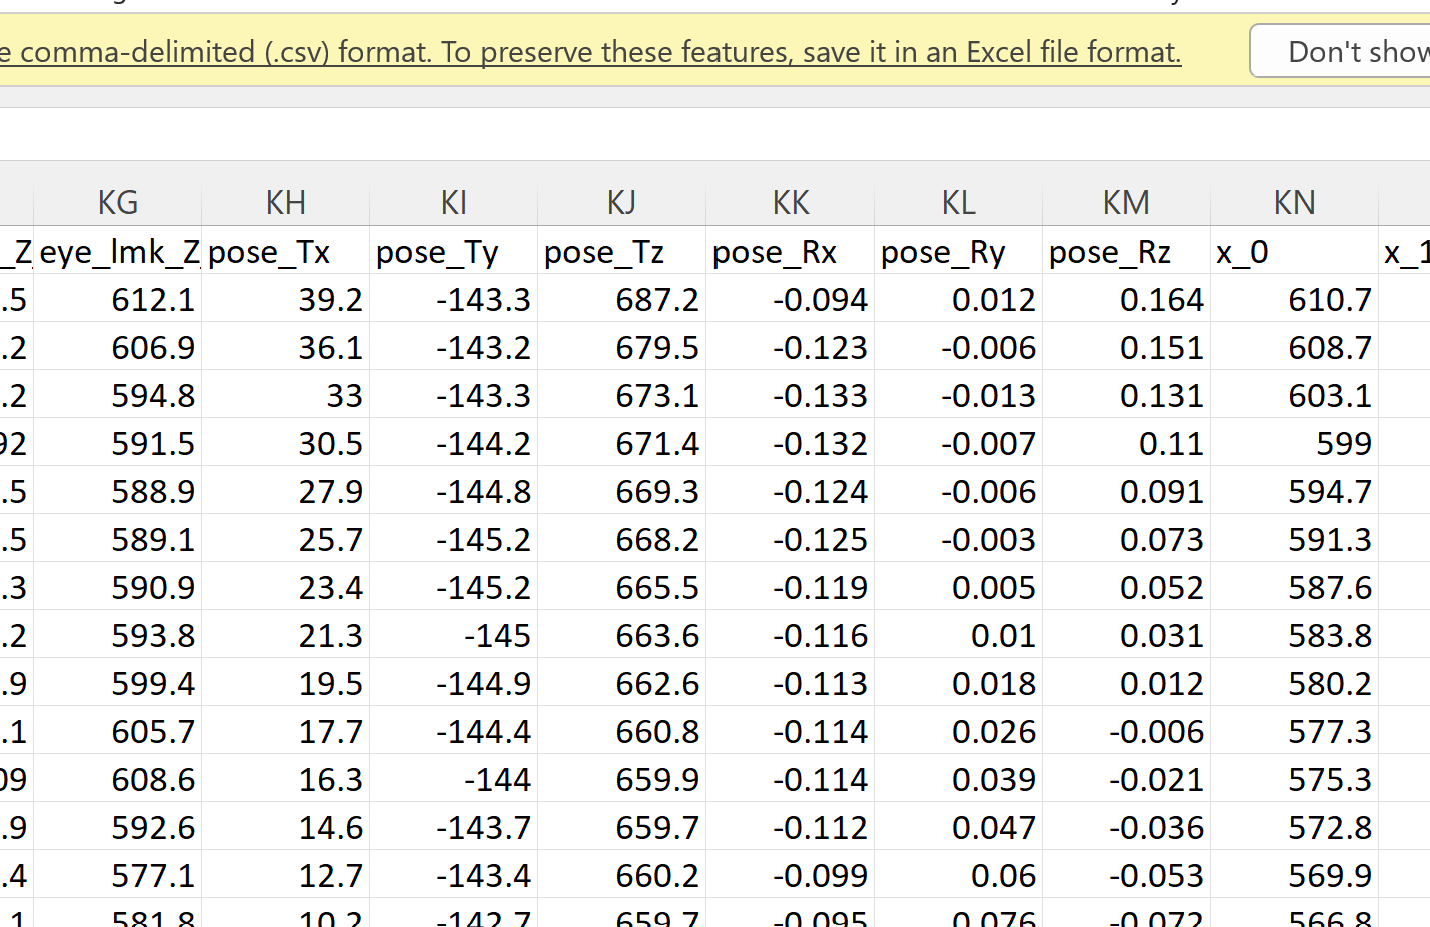
\includegraphics[width=0.75\columnwidth]{figures/openface-csv.png}
    \caption{A Snapshot of OpenFace 2.2~\cite{baltrusaitis_openface_2018} Outputs}
    \label{fig:openface-outputs}
\end{figure}

We then inserted OpenFace 2.2~\cite{baltrusaitis_openface_2018} into the inference pipeline of one of our better performing model variants and attempted to emulate a video chat system, one half at a time. We subjected a ``viewer" video sequence to head pose extraction by OpenFace 2.2 from all frames, as show in figure~\ref{fig:3d-video-chat-rendering-pipeline}. We used one of the utility functions in the single-view MPI modules to extract the yaw, pitch, and roll angles of the ``viewer" frames in a manner conducive to being accepted by the MPI inference. We then rendered the ``viewee" video sequence at the head pose of the ``viewer" frames with matching timestamps. Perhaps more precision could have been added by using not just head pose estimation but also gaze estimation with OpenFace. A snapshot of OpenFace 2.2 outputs for multiple frames in a sequence is shown in figure~\ref{fig:openface-outputs}

